\documentclass[aspectratio=169,11pt]{beamer}

\usepackage[T1]{fontenc}
\usepackage{lmodern}
\usepackage{booktabs}
\usepackage{array}
\usepackage{tikz}
\usetikzlibrary{positioning,arrows.meta,fit}

\definecolor{DeepNavy}{HTML}{13263A}
\definecolor{WarmGold}{HTML}{D9A441}
\definecolor{SoftBlue}{HTML}{EAF1F7}
\definecolor{SoftGold}{HTML}{FFF4D6}
\definecolor{Ink}{HTML}{1E2933}
\definecolor{Muted}{HTML}{5D6B78}
\definecolor{AlertRed}{HTML}{9D2C2C}
\definecolor{Green}{HTML}{2F6F4E}

\setbeamercolor{normal text}{fg=Ink,bg=white}
\setbeamercolor{structure}{fg=DeepNavy}
\setbeamercolor{frametitle}{fg=white,bg=DeepNavy}
\setbeamercolor{title}{fg=white}
\setbeamercolor{subtitle}{fg=SoftBlue}
\setbeamercolor{block title}{fg=white,bg=DeepNavy}
\setbeamercolor{block body}{fg=Ink,bg=SoftBlue}
\setbeamercolor{alertblock title}{fg=white,bg=AlertRed}
\setbeamercolor{alertblock body}{fg=Ink,bg=SoftGold}
\setbeamercolor{exampleblock title}{fg=white,bg=Green}
\setbeamercolor{exampleblock body}{fg=Ink,bg=SoftBlue}
\setbeamercolor{itemize item}{fg=WarmGold}
\setbeamercolor{itemize subitem}{fg=DeepNavy}
\setbeamercolor{enumerate item}{fg=WarmGold}

\setbeamertemplate{navigation symbols}{}
\setbeamertemplate{footline}{%
  \leavevmode%
  \hbox{%
  \begin{beamercolorbox}[wd=.82\paperwidth,ht=2.7ex,dp=1.2ex,leftskip=1em]{author in head/foot}%
    \color{Muted}\small SWOSU Computing Commons \textbullet\ Week 3: Containers + Reproducibility
  \end{beamercolorbox}%
  \begin{beamercolorbox}[wd=.18\paperwidth,ht=2.7ex,dp=1.2ex,rightskip=1em plus1fil]{date in head/foot}%
    \color{Muted}\small \insertframenumber/\inserttotalframenumber
  \end{beamercolorbox}}%
}

\newcommand{\bigquestion}[1]{%
  \begin{center}
  \vspace{0.15em}
  {\Large\bfseries\color{DeepNavy}#1}
  \end{center}
}

\title{It Worked on My Machine}
\subtitle{Repeatability, Reproducibility, Containers, and Evidence}
\author{SWOSU Computing Commons}
\date{Week 3 \textbullet\ Fall 2026}

\begin{document}

{\setbeamercolor{background canvas}{bg=DeepNavy}
\begin{frame}[plain]
  \vspace{1.0cm}
  {\Huge\bfseries\color{white}It Worked on My Machine\par}
  \vspace{0.35cm}
  {\Large\color{SoftBlue}Repeatability, Reproducibility, Containers, and Evidence\par}
  \vfill
  {\large\color{WarmGold}Week 3 question}\par
  \vspace{0.15cm}
  {\Large\color{white}If the code stays the same, what else can change?\par}
  \vfill
  {\small\color{SoftBlue}SWOSU Computing Commons \textbullet\ shared by DSCT and Computer Architecture}
\end{frame}}

\begin{frame}{Start with a prediction}
\bigquestion{Same code. Same input. Same command. Same experiment?}

\begin{center}
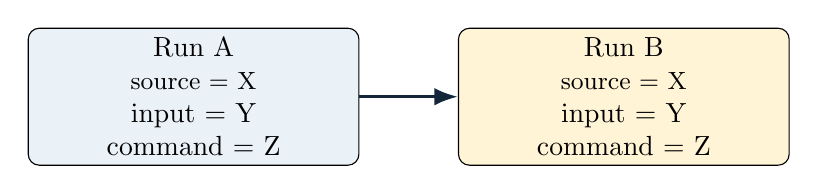
\begin{tikzpicture}[node distance=1.25cm]
  \node[draw,rounded corners,fill=SoftBlue,minimum width=4.2cm,minimum height=1.6cm,align=center] (a) {Run A\\\small source = X\\input = Y\\command = Z};
  \node[draw,rounded corners,fill=SoftGold,right=of a,minimum width=4.2cm,minimum height=1.6cm,align=center] (b) {Run B\\\small source = X\\input = Y\\command = Z};
  \draw[-{Latex[length=3mm]},very thick,DeepNavy] (a) -- (b);
\end{tikzpicture}
\end{center}

\begin{alertblock}{Before we measure}
Write down your prediction: will every observation be identical? Name three pieces of environment context that could matter.
\end{alertblock}
\end{frame}

\begin{frame}{Code is only one layer of the experiment}
\begin{center}
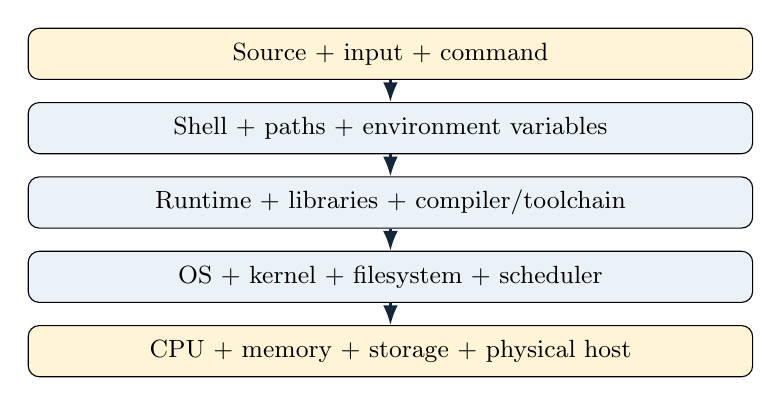
\begin{tikzpicture}[node distance=0.28cm, every node/.style={font=\small}]
  \node[draw,rounded corners,fill=SoftGold,minimum width=9.2cm,minimum height=.65cm] (src) {Source + input + command};
  \node[draw,rounded corners,fill=SoftBlue,below=of src,minimum width=9.2cm,minimum height=.65cm] (shell) {Shell + paths + environment variables};
  \node[draw,rounded corners,fill=SoftBlue,below=of shell,minimum width=9.2cm,minimum height=.65cm] (runtime) {Runtime + libraries + compiler/toolchain};
  \node[draw,rounded corners,fill=SoftBlue,below=of runtime,minimum width=9.2cm,minimum height=.65cm] (os) {OS + kernel + filesystem + scheduler};
  \node[draw,rounded corners,fill=SoftGold,below=of os,minimum width=9.2cm,minimum height=.65cm] (hw) {CPU + memory + storage + physical host};
  \draw[-{Latex[length=2.5mm]},thick,DeepNavy] (src) -- (shell);
  \draw[-{Latex[length=2.5mm]},thick,DeepNavy] (shell) -- (runtime);
  \draw[-{Latex[length=2.5mm]},thick,DeepNavy] (runtime) -- (os);
  \draw[-{Latex[length=2.5mm]},thick,DeepNavy] (os) -- (hw);
\end{tikzpicture}
\end{center}

\begin{block}{The Week 3 problem}
Variation can sneak in at every layer. A useful experiment must say what we held fixed and what we merely observed.
\end{block}
\end{frame}

\begin{frame}{Where can variation sneak in?}
\begin{columns}[T,onlytextwidth]
\column{0.49\textwidth}
\textbf{Software-side variation}
\begin{itemize}
  \item different shell or path rules
  \item different Python / Java / compiler
  \item different package versions
  \item different environment variables
  \item different filesystem contents
\end{itemize}

\column{0.49\textwidth}
\textbf{Host-side variation}
\begin{itemize}
  \item different CPU architecture
  \item different memory available
  \item different kernel behavior
  \item different machine load
  \item different timing and storage behavior
\end{itemize}
\end{columns}

\begin{exampleblock}{Key idea}
``It worked on my machine'' is not an excuse. It is a clue that the experiment had hidden context.
\end{exampleblock}
\end{frame}

\begin{frame}{Control it or record it}
\bigquestion{You cannot freeze the universe. So what do you do?}

\begin{columns}[T,onlytextwidth]
\column{0.48\textwidth}
\begin{block}{CONTROL IT}
Hold a variable fixed when the experiment reasonably can.
\begin{itemize}
  \item source revision
  \item input data
  \item tool versions
  \item entry command
\end{itemize}
\end{block}

\column{0.48\textwidth}
\begin{exampleblock}{RECORD IT}
Preserve context when it cannot or should not be fixed.
\begin{itemize}
  \item executing architecture
  \item kernel / OS identity
  \item timestamp
  \item visible resources
\end{itemize}
\end{exampleblock}
\end{columns}
\end{frame}

\begin{frame}{A reproducibility contract}
\bigquestion{What must another person know to repeat the reasoning task?}

\begin{center}
\begin{tabular}{>{\bfseries}p{3.0cm} p{8.3cm}}
\toprule
Identity & source revision, image identity, or course snapshot \\
Input & the exact file/data used \\
Action & exact command or wrapper \\
Scope & host-visible, WSL-visible, container-visible, etc. \\
Evidence & output shape, receipt, artifact, or measurement \\
Boundary & limitations another person must know \\
\bottomrule
\end{tabular}
\end{center}

\begin{block}{Contract, not incantation}
You do not need to memorize every hidden command. You do need to know what the wrapper promises and what evidence it leaves behind.
\end{block}
\end{frame}

\begin{frame}{A receipt is evidence that survives the terminal}
\begin{columns}[T,onlytextwidth]
\column{0.53\textwidth}
A useful receipt can preserve:
\begin{itemize}
  \item source/tool identity
  \item execution scope
  \item relevant environment facts
  \item input/output identity
  \item timestamp or run identity
  \item pass/fail plus a reason
\end{itemize}

\column{0.43\textwidth}
\begin{alertblock}{Do not overclaim}
A receipt records what happened. It does not automatically prove \textbf{why} it happened.
\end{alertblock}
\end{columns}

\vspace{0.35cm}
\begin{center}
\Large\bfseries Observation $\neq$ explanation
\end{center}
\end{frame}

\begin{frame}{So what is a container?}
\bigquestion{Could we put part of the experiment in a controlled box?}

\begin{center}
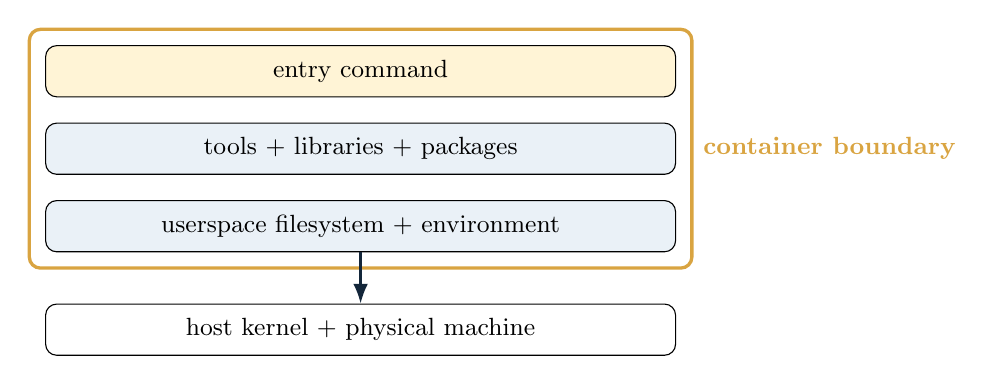
\begin{tikzpicture}[every node/.style={font=\small},node distance=.32cm]
  \node[draw,rounded corners,fill=SoftGold,minimum width=8.0cm,minimum height=.65cm] (entry) {entry command};
  \node[draw,rounded corners,fill=SoftBlue,below=of entry,minimum width=8.0cm,minimum height=.65cm] (tools) {tools + libraries + packages};
  \node[draw,rounded corners,fill=SoftBlue,below=of tools,minimum width=8.0cm,minimum height=.65cm] (fs) {userspace filesystem + environment};
  \node[draw,rounded corners,fill=white,below=0.65cm of fs,minimum width=8.0cm,minimum height=.65cm] (kernel) {host kernel + physical machine};
  \node[draw=WarmGold,very thick,rounded corners,fit=(entry)(tools)(fs),inner sep=.2cm,label={[WarmGold]right:\bfseries container boundary}] {};
  \draw[-{Latex[length=2.5mm]},thick,DeepNavy] (fs) -- (kernel);
\end{tikzpicture}
\end{center}

\begin{block}{Our Week 3 reason}
We use a container so we can hold more of the \textbf{software environment} constant while deliberately observing what still depends on the host.
\end{block}
\end{frame}

\begin{frame}{Image vs. running container}
\begin{columns}[T,onlytextwidth]
\column{0.47\textwidth}
\begin{block}{IMAGE}
A frozen template that describes the environment we want.
\begin{itemize}
  \item tools
  \item packages
  \item filesystem
  \item default command
\end{itemize}
\end{block}

\column{0.47\textwidth}
\begin{exampleblock}{CONTAINER}
A running instance created from that image.
\begin{itemize}
  \item starts
  \item performs work
  \item can be discarded
  \item does not erase the image
\end{itemize}
\end{exampleblock}
\end{columns}

\begin{alertblock}{Vocabulary worth keeping}
Image = template. Container = disposable running instance.
\end{alertblock}
\end{frame}

\begin{frame}{Pinned identity beats ``latest''}
\bigquestion{What happens if the environment silently changes next week?}

\begin{columns}[T,onlytextwidth]
\column{0.47\textwidth}
\begin{alertblock}{Floating tag}
\texttt{:latest}
\begin{itemize}
  \item easy to type
  \item may point somewhere new later
  \item weak evidence for reproduction
\end{itemize}
\end{alertblock}

\column{0.47\textwidth}
\begin{exampleblock}{Pinned identity}
Digest / fixed version
\begin{itemize}
  \item identifies one exact image
  \item does not silently drift
  \item stronger reproducibility contract
\end{itemize}
\end{exampleblock}
\end{columns}
\end{frame}

\begin{frame}{Your files can cross the boundary}
\bigquestion{How does your work get into the container and back out?}

\begin{center}
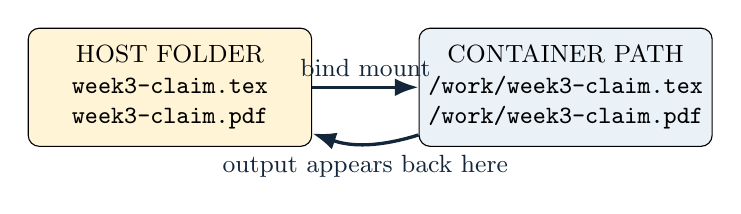
\begin{tikzpicture}[node distance=1.0cm and 1.35cm,every node/.style={font=\small,align=center}]
  \node[draw,rounded corners,fill=SoftGold,minimum width=3.6cm,minimum height=1.5cm] (host) {HOST FOLDER\\\texttt{week3-claim.tex}\\\texttt{week3-claim.pdf}};
  \node[draw,rounded corners,fill=SoftBlue,right=of host,minimum width=3.6cm,minimum height=1.5cm] (container) {CONTAINER PATH\\\texttt{/work/week3-claim.tex}\\\texttt{/work/week3-claim.pdf}};
  \draw[-{Latex[length=3mm]},very thick,DeepNavy] (host) -- node[above]{bind mount} (container);
  \draw[-{Latex[length=3mm]},very thick,DeepNavy] (container) to[bend left=18] node[below]{output appears back here} (host);
\end{tikzpicture}
\end{center}

\begin{block}{One file, two path names}
The file lives on the host, but the container sees that mounted folder at its own path. Confusing host paths and container paths is a normal, diagnosable mistake.
\end{block}
\end{frame}

\begin{frame}{What containers help control}
\begin{columns}[T,onlytextwidth]
\column{0.48\textwidth}
\begin{exampleblock}{Often controlled well}
\begin{itemize}
  \item userspace filesystem
  \item installed packages
  \item tool versions
  \item environment variables
  \item entry command
  \item known working directory
\end{itemize}
\end{exampleblock}

\column{0.48\textwidth}
\begin{alertblock}{Still inherited / variable}
\begin{itemize}
  \item physical CPU
  \item host kernel
  \item host load and scheduling
  \item storage hardware
  \item timing noise
  \item every possible platform quirk
\end{itemize}
\end{alertblock}
\end{columns}
\end{frame}

\begin{frame}{Containers do not make machines identical}
\bigquestion{Two containers can share an image and still observe different hosts.}

\begin{center}
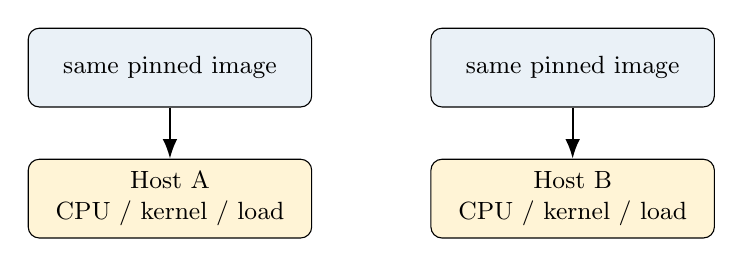
\begin{tikzpicture}[node distance=.65cm and 1.5cm,every node/.style={font=\small,align=center}]
  \node[draw,rounded corners,fill=SoftBlue,minimum width=3.6cm,minimum height=1.0cm] (ca) {same pinned image};
  \node[draw,rounded corners,fill=SoftBlue,right=of ca,minimum width=3.6cm,minimum height=1.0cm] (cb) {same pinned image};
  \node[draw,rounded corners,fill=SoftGold,below=of ca,minimum width=3.6cm,minimum height=1.0cm] (ha) {Host A\\CPU / kernel / load};
  \node[draw,rounded corners,fill=SoftGold,below=of cb,minimum width=3.6cm,minimum height=1.0cm] (hb) {Host B\\CPU / kernel / load};
  \draw[-{Latex[length=2.5mm]},thick] (ca) -- (ha);
  \draw[-{Latex[length=2.5mm]},thick] (cb) -- (hb);
\end{tikzpicture}
\end{center}

\begin{alertblock}{Bad claim}
``The container makes both computers the same.''
\end{alertblock}
\begin{exampleblock}{Better claim}
``The container fixes more of the software environment, making remaining host-dependent differences easier to identify.''
\end{exampleblock}
\end{frame}

\begin{frame}{The known-good run}
\bigquestion{First prove the supplied environment can do one tiny job.}

\begin{enumerate}
  \item Start with the course-provided source.
  \item Run the course-provided wrapper.
  \item Read the image, host path, container path, source, output, and result lines.
  \item Open the produced artifact.
  \item Confirm the artifact actually reflects the source you ran.
\end{enumerate}

\begin{block}{For DSCT}
The tiny job is a \texttt{.tex} claim/proof compiled into a PDF. The wrapper handles the container command; your job is to understand the contract and verify the artifact.
\end{block}
\end{frame}

\begin{frame}{Then perturb it on purpose}
\bigquestion{A system you can only use when nothing goes wrong is not yet a tool.}

\begin{center}
\Large\bfseries
PERTURB $\rightarrow$ DIAGNOSE $\rightarrow$ PROPOSE $\rightarrow$ RERUN $\rightarrow$ VERIFY
\end{center}

\vspace{0.45cm}
\begin{columns}[T,onlytextwidth]
\column{0.48\textwidth}
Common bounded failures:
\begin{itemize}
  \item wrong host path
  \item missing source file
  \item runtime/image problem
  \item content/tool error
\end{itemize}

\column{0.48\textwidth}
Evidence habits:
\begin{itemize}
  \item read the reason first
  \item classify before changing things
  \item AI suggestions are proposals
  \item rerun after the repair
  \item inspect the real artifact
\end{itemize}
\end{columns}
\end{frame}

\begin{frame}{Native vs. container is an experiment}
\begin{center}
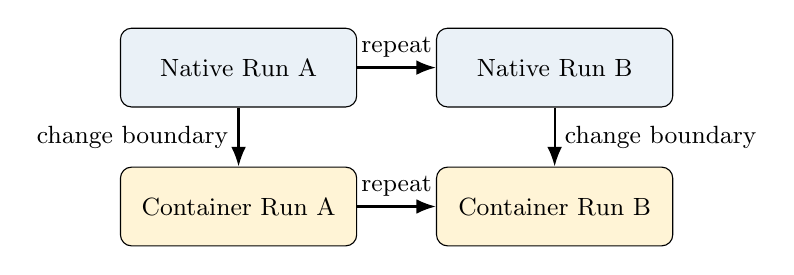
\begin{tikzpicture}[node distance=.75cm and 1.0cm,every node/.style={font=\small,align=center}]
  \node[draw,rounded corners,fill=SoftBlue,minimum width=3.0cm,minimum height=1.0cm] (n1) {Native Run A};
  \node[draw,rounded corners,fill=SoftBlue,right=of n1,minimum width=3.0cm,minimum height=1.0cm] (n2) {Native Run B};
  \node[draw,rounded corners,fill=SoftGold,below=of n1,minimum width=3.0cm,minimum height=1.0cm] (c1) {Container Run A};
  \node[draw,rounded corners,fill=SoftGold,right=of c1,minimum width=3.0cm,minimum height=1.0cm] (c2) {Container Run B};
  \draw[-{Latex[length=2.5mm]},thick] (n1) -- node[above]{repeat} (n2);
  \draw[-{Latex[length=2.5mm]},thick] (c1) -- node[above]{repeat} (c2);
  \draw[-{Latex[length=2.5mm]},thick] (n1) -- node[left]{change boundary} (c1);
  \draw[-{Latex[length=2.5mm]},thick] (n2) -- node[right]{change boundary} (c2);
\end{tikzpicture}
\end{center}

\begin{block}{Questions worth asking}
What stays stable? What changes? Which changes are expected? Which differences matter to the claim you are trying to make?
\end{block}
\end{frame}

\begin{frame}{Repeatability and reproducibility are not the same claim}
\begin{columns}[T,onlytextwidth]
\column{0.47\textwidth}
\begin{block}{REPEATABILITY}
Can I perform the same procedure again in the same environment and obtain the required evidence shape?
\end{block}

\column{0.47\textwidth}
\begin{exampleblock}{REPRODUCIBILITY}
Can another environment preserve the important contract well enough to reproduce the reasoning or result?
\end{exampleblock}
\end{columns}

\vspace{0.35cm}
\begin{alertblock}{Neither means}
``Every bit of both machines was identical.''
\end{alertblock}
\end{frame}

\begin{frame}{Make only the claim your evidence can carry}
\begin{block}{A bounded claim}
The same \underline{\hspace{2.0cm}} and \underline{\hspace{2.0cm}} produced \underline{\hspace{2.5cm}} across repeated runs. The receipt describes \underline{\hspace{2.7cm}}, but it does not prove \underline{\hspace{2.7cm}}.
\end{block}

\vspace{0.45cm}
\begin{columns}[T,onlytextwidth]
\column{0.48\textwidth}
\textbf{Ask yourself}
\begin{itemize}
  \item What did I actually observe?
  \item What did I control?
  \item What did I merely record?
\end{itemize}

\column{0.48\textwidth}
\textbf{Then state}
\begin{itemize}
  \item one supported conclusion
  \item one limitation
  \item one thing more evidence would decide
\end{itemize}
\end{columns}
\end{frame}

\begin{frame}{One lesson, two course lenses}
\begin{center}
\begin{tabular}{>{\bfseries}p{2.6cm} p{4.5cm} p{4.5cm}}
\toprule
 & DSCT & Computer Architecture \\
\midrule
Main question & What claim can the evidence justify? & What environment/machine layer changed? \\
Receipt & What does it prove and not prove? & What did the process actually observe? \\
Container & How much confidence does the boundary buy? & Which layers moved inside/outside the boundary? \\
Difference & Is it relevant to the argument? & Why might the value legitimately differ? \\
\bottomrule
\end{tabular}
\end{center}
\end{frame}

\begin{frame}{Your Week 3 mission}
\begin{enumerate}
  \item \textbf{Predict} what environment context might matter.
  \item \textbf{Run} a known-good task and preserve a receipt.
  \item \textbf{Inspect} the container boundary and the artifact it produced.
  \item \textbf{Perturb} one bounded thing and recover from the failure.
  \item \textbf{Compare} what stayed stable and what changed.
  \item \textbf{Defend} one claim that your evidence genuinely supports.
\end{enumerate}

\begin{exampleblock}{The point is not container syntax}
The point is learning to make a computing result easier to reproduce, inspect, diagnose, and defend.
\end{exampleblock}
\end{frame}

{\setbeamercolor{background canvas}{bg=DeepNavy}
\begin{frame}[plain]
\vfill
\begin{center}
{\Huge\bfseries\color{white}Same code is not the same experiment.\par}
\vspace{0.55cm}
{\Large\color{WarmGold}Control what you can.\par}
\vspace{0.22cm}
{\Large\color{SoftBlue}Record what you cannot.\par}
\vspace{0.22cm}
{\Large\color{white}Make only the claim your evidence can carry.\par}
\end{center}
\vfill
\end{frame}}

\end{document}
